\documentclass[tikz,border=3pt]{standalone}
\usepackage[utf8]{inputenc}
\usepackage[T1]{fontenc}
\usepackage{lmodern}
\renewcommand{\familydefault}{\sfdefault}
\usepackage{sansmath}\sansmath
\usepackage{chemfig}
\usepackage{pgfplots}\pgfplotsset{compat=1.18,/pgf/number format/use comma,/pgf/number format/1000 sep={.}}
\usetikzlibrary{arrows.meta,calc,positioning,decorations.pathmorphing,patterns}
% paleta del sitio
\definecolor{nar}{HTML}{E8680C}\definecolor{narc}{HTML}{FFB35C}\definecolor{hielo}{HTML}{FFF3E8}
\definecolor{tinta}{HTML}{1D1D1F}\definecolor{gris}{HTML}{6E6E73}\definecolor{lila}{HTML}{7C5CF0}
\definecolor{azul}{HTML}{2F6FD6}\definecolor{menta}{HTML}{17A673}\definecolor{coral}{HTML}{E8342A}
\begin{document}
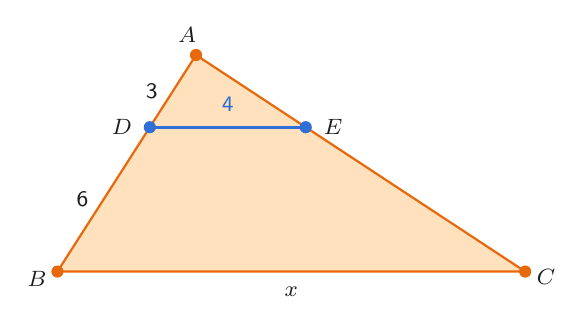
\begin{tikzpicture}[font=\small,x=0.55cm,y=0.55cm,line cap=round,line join=round,step={(1,1)}]
\filldraw[fill=narc!40,draw=nar,thick] (3.2,5.0)--(0,0)--(10.8,0)--cycle;
\fill[nar] (3.2,5.0) circle (2.2pt);
\node[font=\footnotesize,text=tinta,inner sep=0pt] at ($(3.2,5.0)+(114:0.5)$) {$A$};
\fill[nar] (0,0) circle (2.2pt);
\node[font=\footnotesize,text=tinta,inner sep=0pt] at ($(0,0)+(-160:0.5)$) {$B$};
\fill[nar] (10.8,0) circle (2.2pt);
\node[font=\footnotesize,text=tinta,inner sep=0pt] at ($(10.8,0)+(-15:0.5)$) {$C$};
\draw[azul,very thick] (2.133,3.333)--(5.733,3.333);
\fill[azul] (2.133,3.333) circle (2.2pt) node[left=3pt,font=\footnotesize,text=tinta] {$D$};
\fill[azul] (5.733,3.333) circle (2.2pt) node[right=3pt,font=\footnotesize,text=tinta] {$E$};
\path (3.2,5.0)--(2.1333333333333337,3.333333333333333) node[midway,left=2pt,font=\footnotesize,text=tinta] {3};
\path (2.1333333333333337,3.333333333333333)--(0,0) node[midway,left=2pt,font=\footnotesize,text=tinta] {6};
\path (2.1333333333333337,3.333333333333333)--(5.733333333333334,3.333333333333333) node[midway,above=2pt,font=\footnotesize,text=azul] {4};
\path (0,0)--(10.8,0) node[midway,below=2pt,font=\footnotesize,text=tinta] {$x$};
\end{tikzpicture}
\end{document}
